%===================================== CHAP 5 =================================
\chapter{Bayesian Q Learning}{\label{ch:bdqn}}

In an attempt to find a better balance between exploration and exploitation this thesis investigates the use of bayesian methods to allow for Thompson sampling. This chapter builds and compares bayesian methods in a linear model context before attempting to extend the most successful methods to neural networks.

\section{Linear Q learning}

In linear Q learning the goal is to create a regression model that maps the state and action to a Q-value, $Q(s,a)$. Let $x_t$ denote the state and action at timestep $t$. $X$ then denotes the design matrix containing these features and $Q$ the vector of corresponding Q-values. The regression model can then be defined as

\begin{equation*}
	Q = X\beta + \varepsilon \quad \text{where} \quad \varepsilon \sim N(0,\sigma^2)
\end{equation*}

with the response value defined as 

\begin{equation}
    \label{eq:q_target}
	Q(s,a) = r_t + \argmax_{a'}Q(s',a').
\end{equation}

The ordinary least squares solution to the $\beta$ coefficients can then be found using the normal equation which in matrix form is

\begin{equation*}
	\beta = [X^TX]^{-1}X^TQ
\end{equation*}

Given this model the agent can take an action by acting greedily over the models $Q(s,a)$ values in a given state. Since this purely an exploitation strategy, it is often coupled with the $\varepsilon$-greedy policy.

\section{Bayesian Linear Q learning}

To extend linear Q learning methods to follow a Thompson sampling policy a bayesian perspective is required. In a RL perspective the goal is to model the posterior

\begin{equation*}
p(Q|\theta, X_{t}) \propto p(\theta|X_{t}, A_{t}, R, X_{t+1})p(\theta)
\end{equation*}

where $Q$ is a vector of all Q-values given the state $X_t$ and $\theta$ denotes all parameters.

The calculation of an arbitrary posterior is computationally heavy which is ill-suited to the already long running reinforcement learning methods. To keep computation costs low this thesis will only consider conjugate priors which have an analytical solution.

\subsection{Normal Prior with Known noise}

There are multiple ways to setup a bayesian regression model using conjugate priors. First consider the case used in \cite{azziz_2018} which creates one model per action and assumes the noise variance is known. The known noise variance is then treated as a hyperparameter. In this case the posterior can be expressed as 

$$
p(\beta_a|\sigma_{\varepsilon_a}, X_{t}, A_{t}, R, X_{t+1}) \propto p(Q_a|\beta_a, \sigma_{\varepsilon_a}, X_{t})p(\beta_a)
$$

In literature it is common to use a gaussian prior for $\beta$

$$
	  p(\beta) = \text{N}(\mu, \sigma_\varepsilon\Lambda^{-1}) 
$$

where $\Lambda$ is the precision matrix. This results in the following posterior update

\begin{align*}
	\Lambda_n & = X^TX + \Lambda_0 \\
	\mu_n     & = \Lambda_n^{-1}(\Lambda_0\mu_0 + X^TQ_a)
\end{align*}

To calculate the target $Q$-value the MAP estimate of $\beta$ is used which in this case is $\mu$. 

\subsection{Normal Prior with Unknown noise}

To avoid the noise variance as a hyperparameter it can be included as an unknown parameter.

$$
p(\beta_a, \sigma_{\varepsilon_a}| X_{t}, A_{t}, R, X_{t+1})\propto p(Q_a|\beta_a, \sigma_{\varepsilon_a}, X_{t})p(\beta_a|\sigma^2_{\varepsilon_a}) p(\sigma^2_{\varepsilon_a})
$$

The conjugate priors for this setup are

\begin{align*}
    & p(\sigma^2) = \text{InvGamma}(\alpha, b)          \\
    & p(\beta|\sigma^2) = \text{N}(\mu, \sigma^2\Sigma) 
\end{align*}

with the posterior update

\begin{align*}
	\Lambda_n & = (X^TX + \Lambda_0)                                         \\
	\mu_n     & = \Lambda_n^{-1}(\Lambda_0\mu_0 + X^TQ)                      \\
	\alpha_n  & = \alpha_0 + \frac{n}{2}                                     \\
	b_n       & = b_0 + (Q^TQ + \mu^T\Lambda_0\mu_0 - \mu_n^T\Lambda_n\mu_n) 
\end{align*}

Once again $\mu$, the MAP estimate of $\beta$ is used to calculate the target Q-value.

\todo: Insert results for linear methods on chain environment?

\begin{figure}[H]
    \centering
    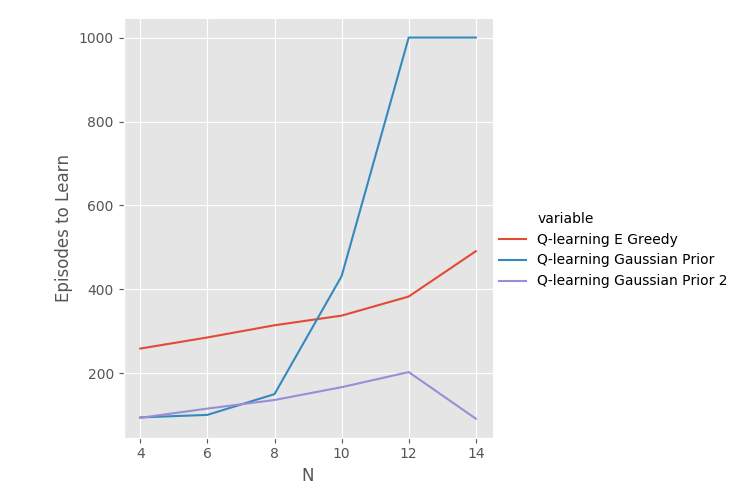
\includegraphics[width=0.8\textwidth]{results_no_prop.png}
    \caption{WIP: \textbf{Performance on chain environment} Guassian Prior 2 includes the noise as a parameter}
    \label{fig:results_no_propr}
\end{figure}


\subsection{Propagating Uncertainty}

One possible issue with the two above methods is training using the MAP estimate of $\beta$. Using the MAP estimate means that the targets come from the following process:

$$
y = R + \max_a X_{t+1}\mu_a.
$$

Though this does incorporate the variance in the reward process through $R$ it does not convey the variance in the Q-value estimate of the next state. Even in a deterministic environment the policy shifts during training mean that there is an uncertainty in the Q-value of the next state. Quoting \cite{moerland_2017},  "\dots repeatedly visiting a state-action pair should not makes us certain about its value if we are still uncertain about what to do next."

One possible method to include this uncertainty is to sample the $\beta$ posterior when calculating the target value.

\todo Here is where I want stronger argumentation of why this should work (other than intuition).

\todo Insert results for linear methods on chain environment

\begin{figure}[H]
    \centering
    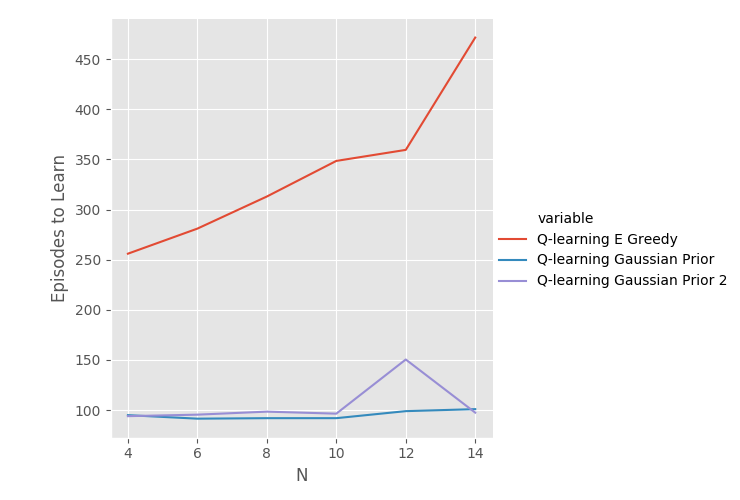
\includegraphics[width=0.8\textwidth]{results_with_prop.png}
    \caption{WIP: \textbf{Performance on chain environment} Guassian Prior 2 includes the noise as a parameter}
    \label{fig:results_no_propr}
\end{figure}

\subsection{Investigating propagation}

To ensure that these methods are propagating uncertainty we can consider a simple example from \cite{osband_2018}. Consider a MPD with two states. The initial state allows only one action that deterministicly leads to state 2 with no reward. State 2 is a terminal state with a known posterior distribution.

If a RL method properly propagates uncertainty the posterior distribution of state 1 should match state 2 as long as $\gamma=1$. To test the following setup was usedThe priors for the known noise models were set to

\begin{align*}
    \beta &\sim N(0,10^3)\\
    \sigma^2 &= 1
\end{align*}

and the priors for the unknown noise models were set to

\begin{align*}
    \beta &\sim N(0,10^3) \\
    \sigma^2 &\sim InvGamma(1,1).
\end{align*}

Three MDP's were set up with a known posterior of $N(1, 0.1), N(1, 1)$ and $N(1, 10)$ respectively. The results are seen in figure \ref{fig:proptest}.

\begin{figure}[H]
    \centering
    \subfloat[$N(1,0.1^2)$]{
        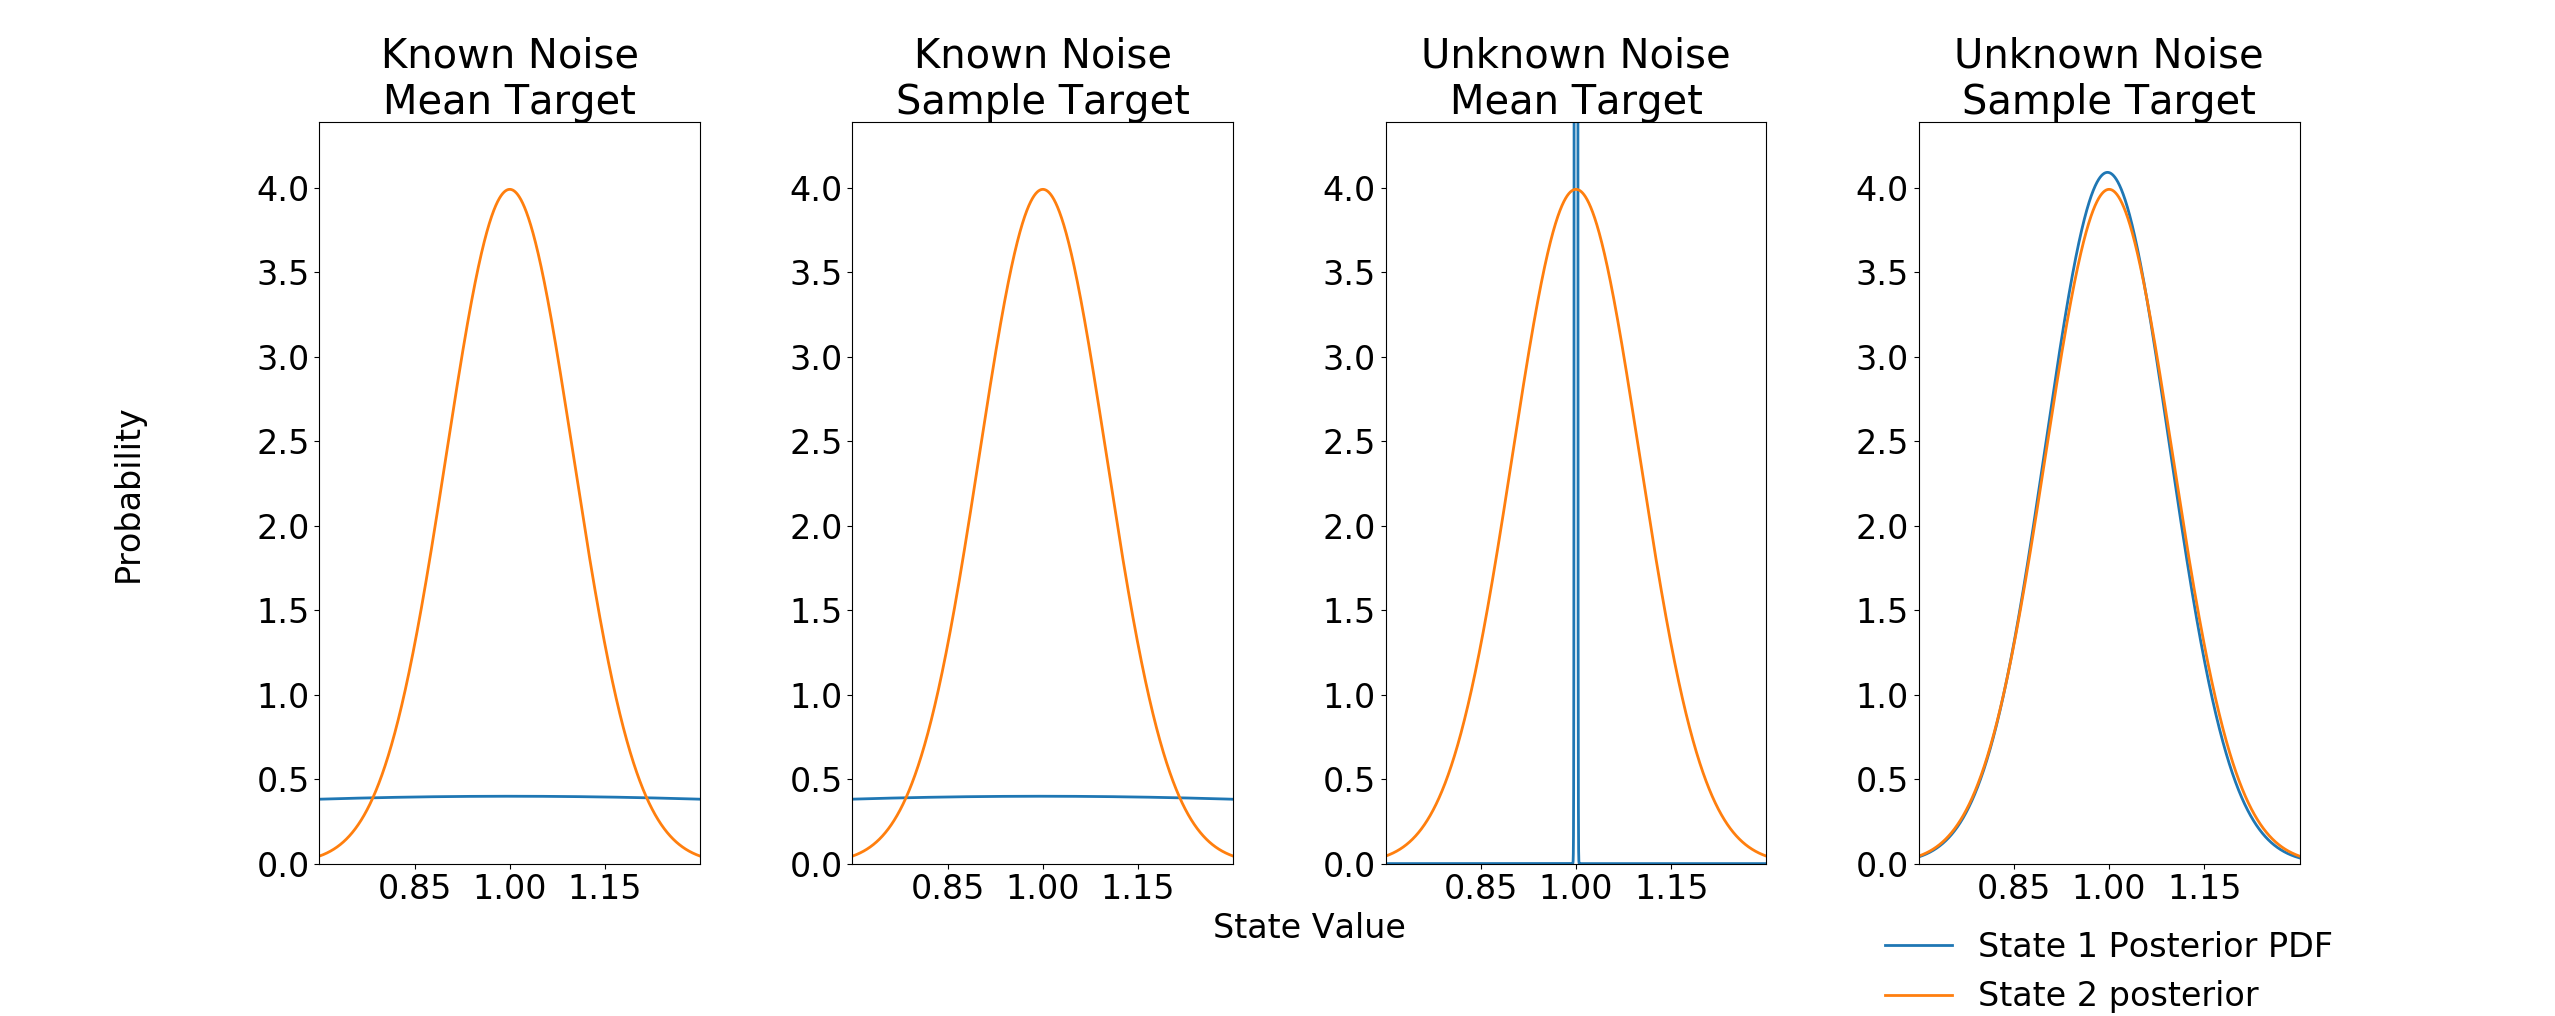
\includegraphics[width=0.5\textwidth]{1000iterationsSD01.png}
    }
    \subfloat[$N(1,1^2)$]{
        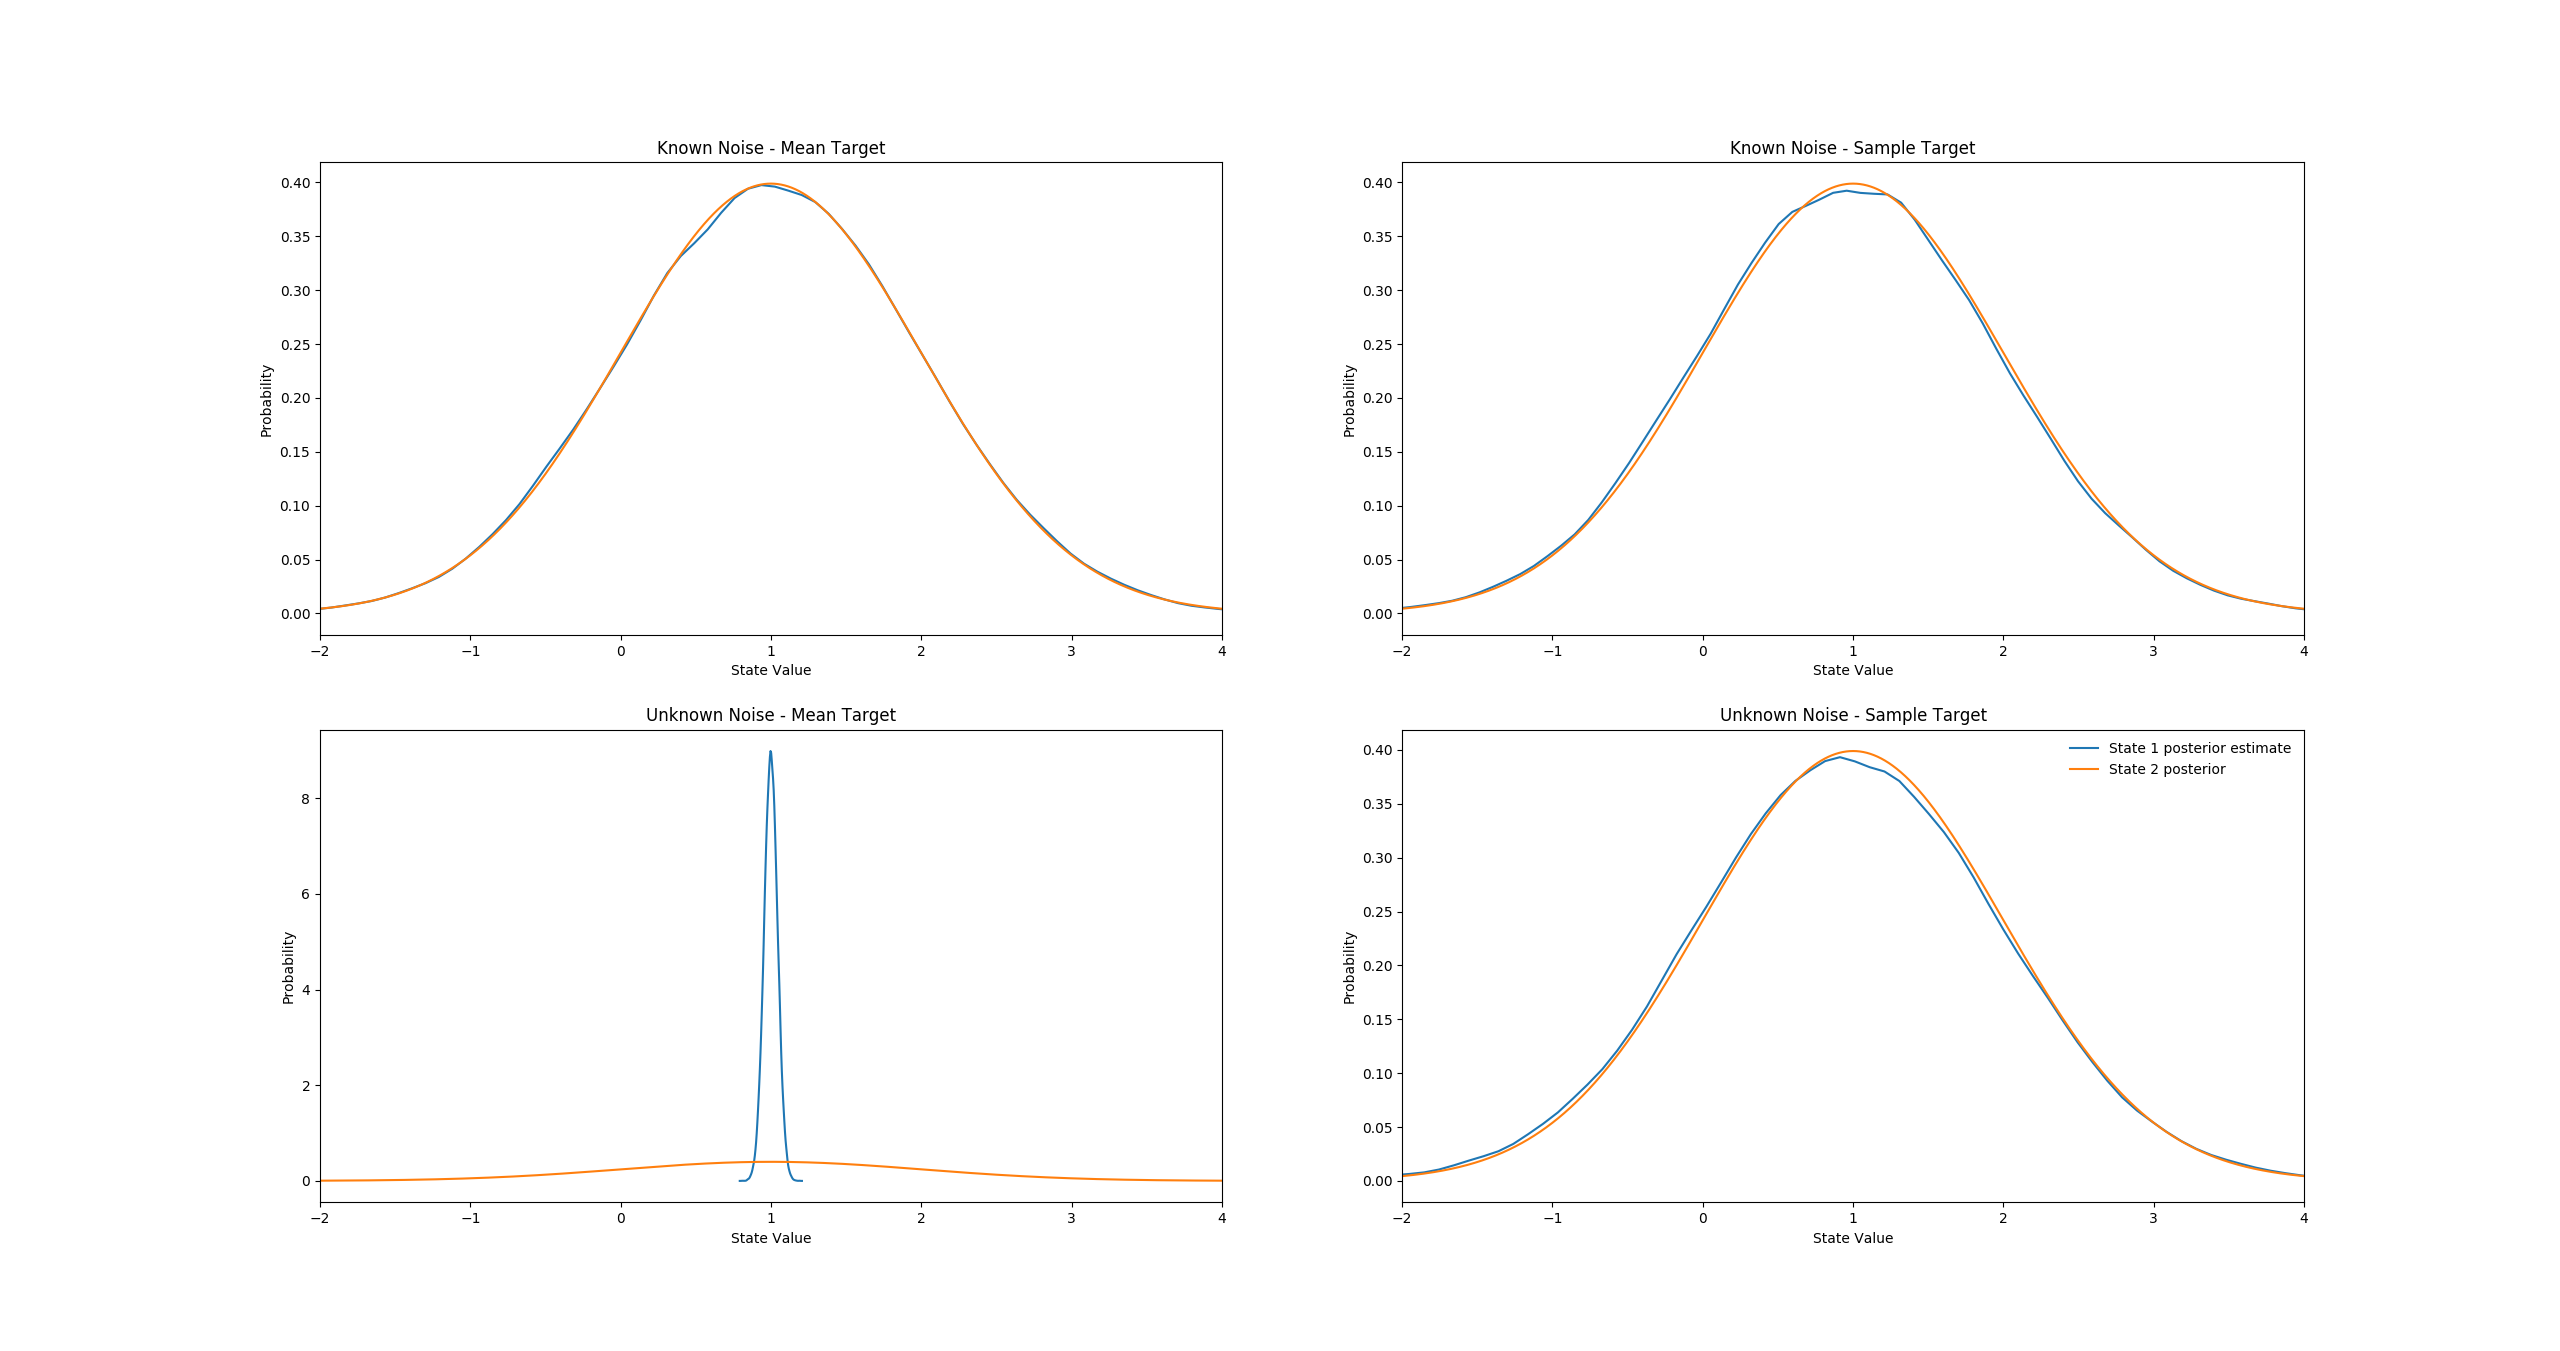
\includegraphics[width=0.5\textwidth]{1000iterationsSD1.png}
    }
    \\
    \subfloat[$N(1,10^2)$]{
        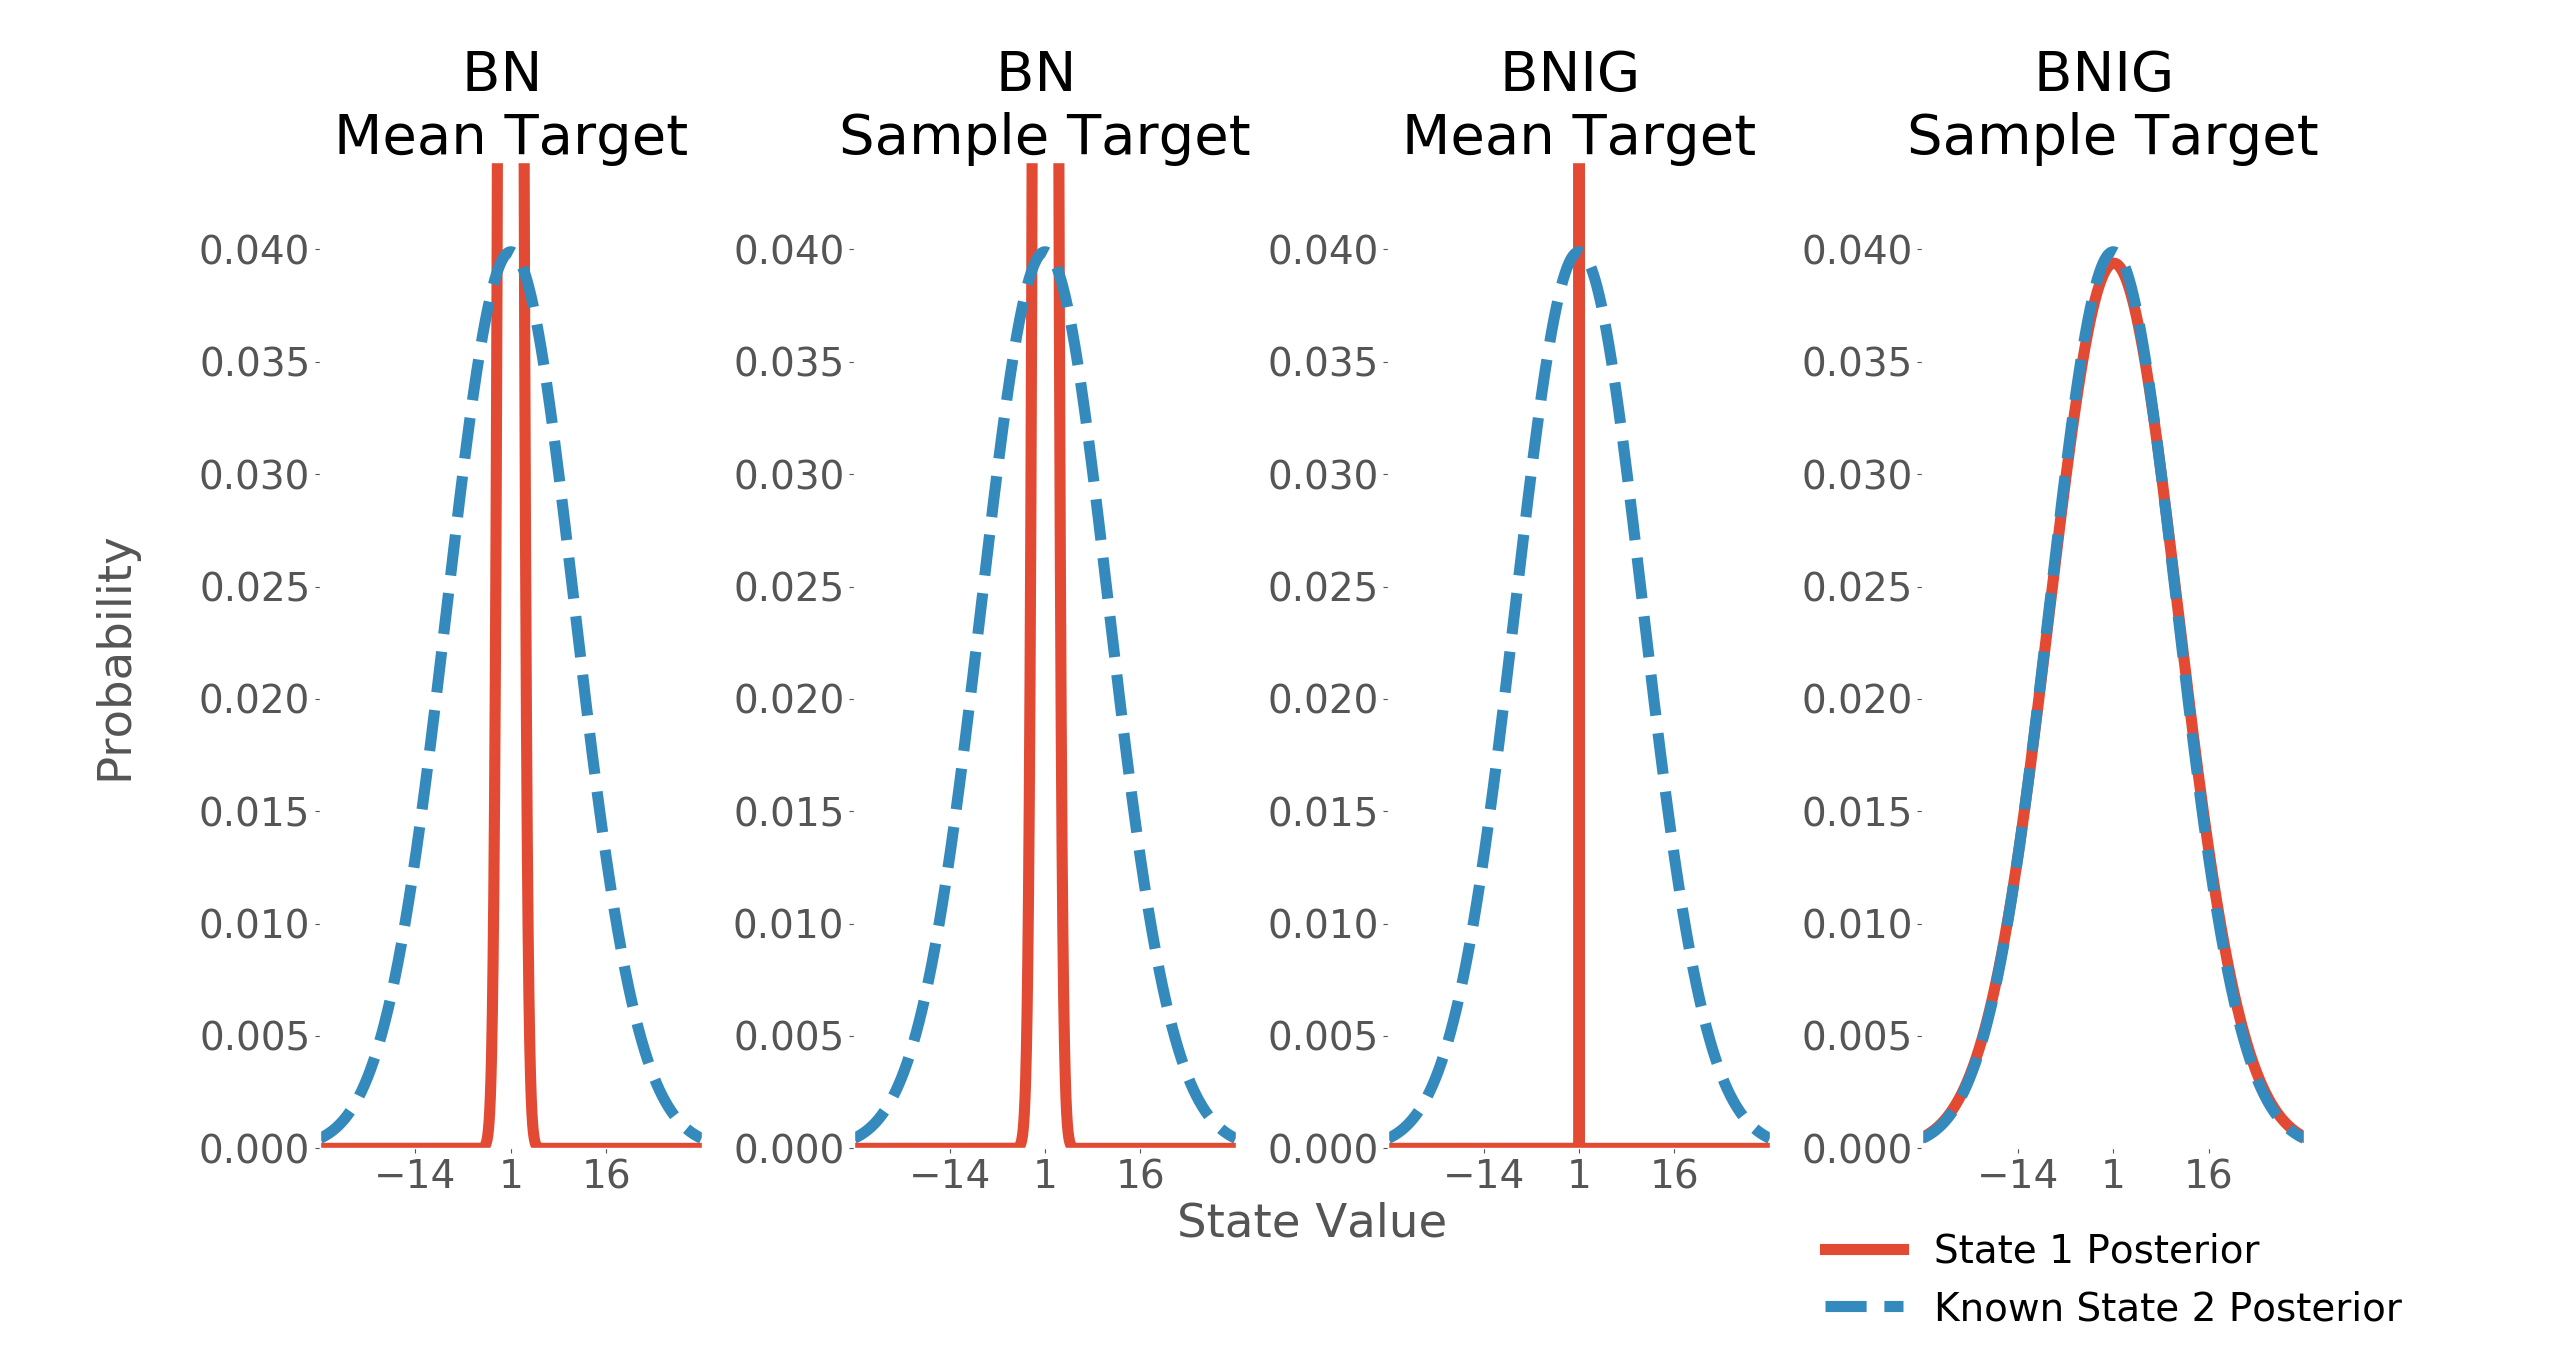
\includegraphics[width=0.5\textwidth]{1000iterationsSD10.png}
    }
    \caption{\textbf{Variance Propagation On 2 State Toy Example}: The known noise models only work if the "known" noise is exactly the noise in the MDP. The unknown noise model seems is the only model that seems to correctly propagate the variance if the target is sampled.}
    \label{fig:proptest}
\end{figure}

Based on these results focus is placed on the unknown noise model with sampled targets. Now consider a modification to the environment where an extra state is placed between the initial and terminal state. This state has the same dynamics meaning it deterministic transitions to the terminal state with zero reward over the transition. This allows an investigation over how well variance is propagated through multiple states.

\begin{figure}[H]
    \centering

    \subfloat[$N(1,1^2)$]{
        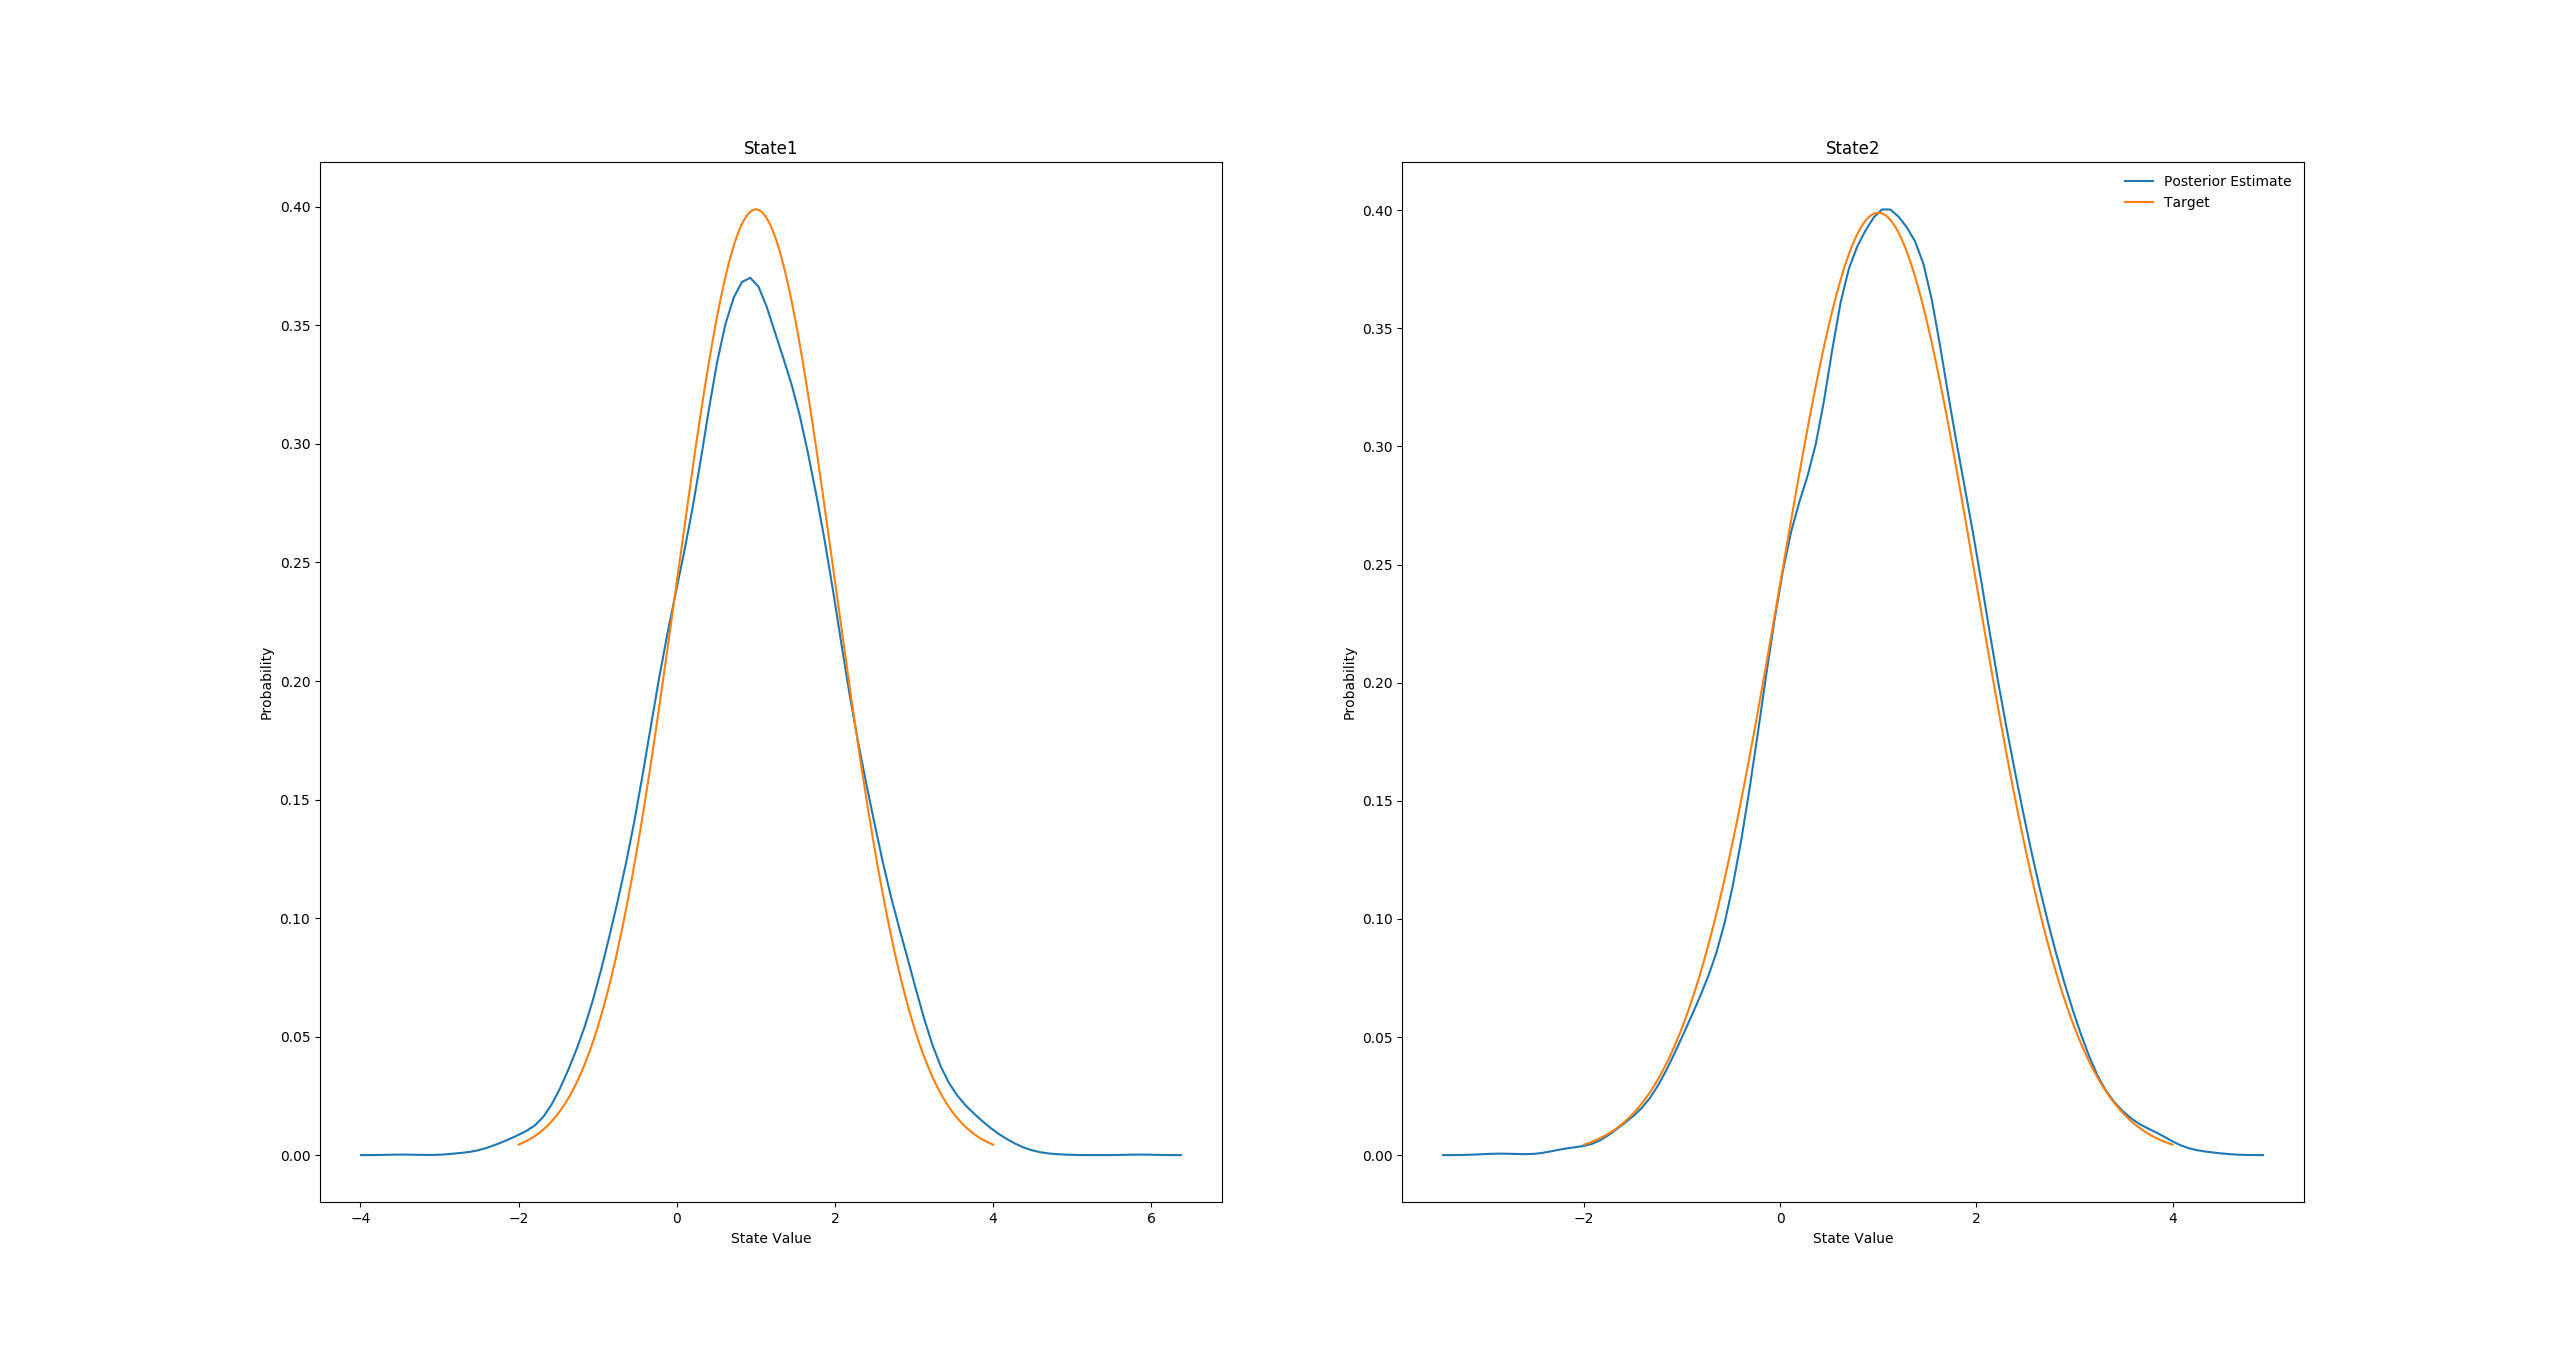
\includegraphics[width=0.5\textwidth]{3State1000iterationsSD1.png}
    }
    \subfloat[$N(1,10^2)$]{
        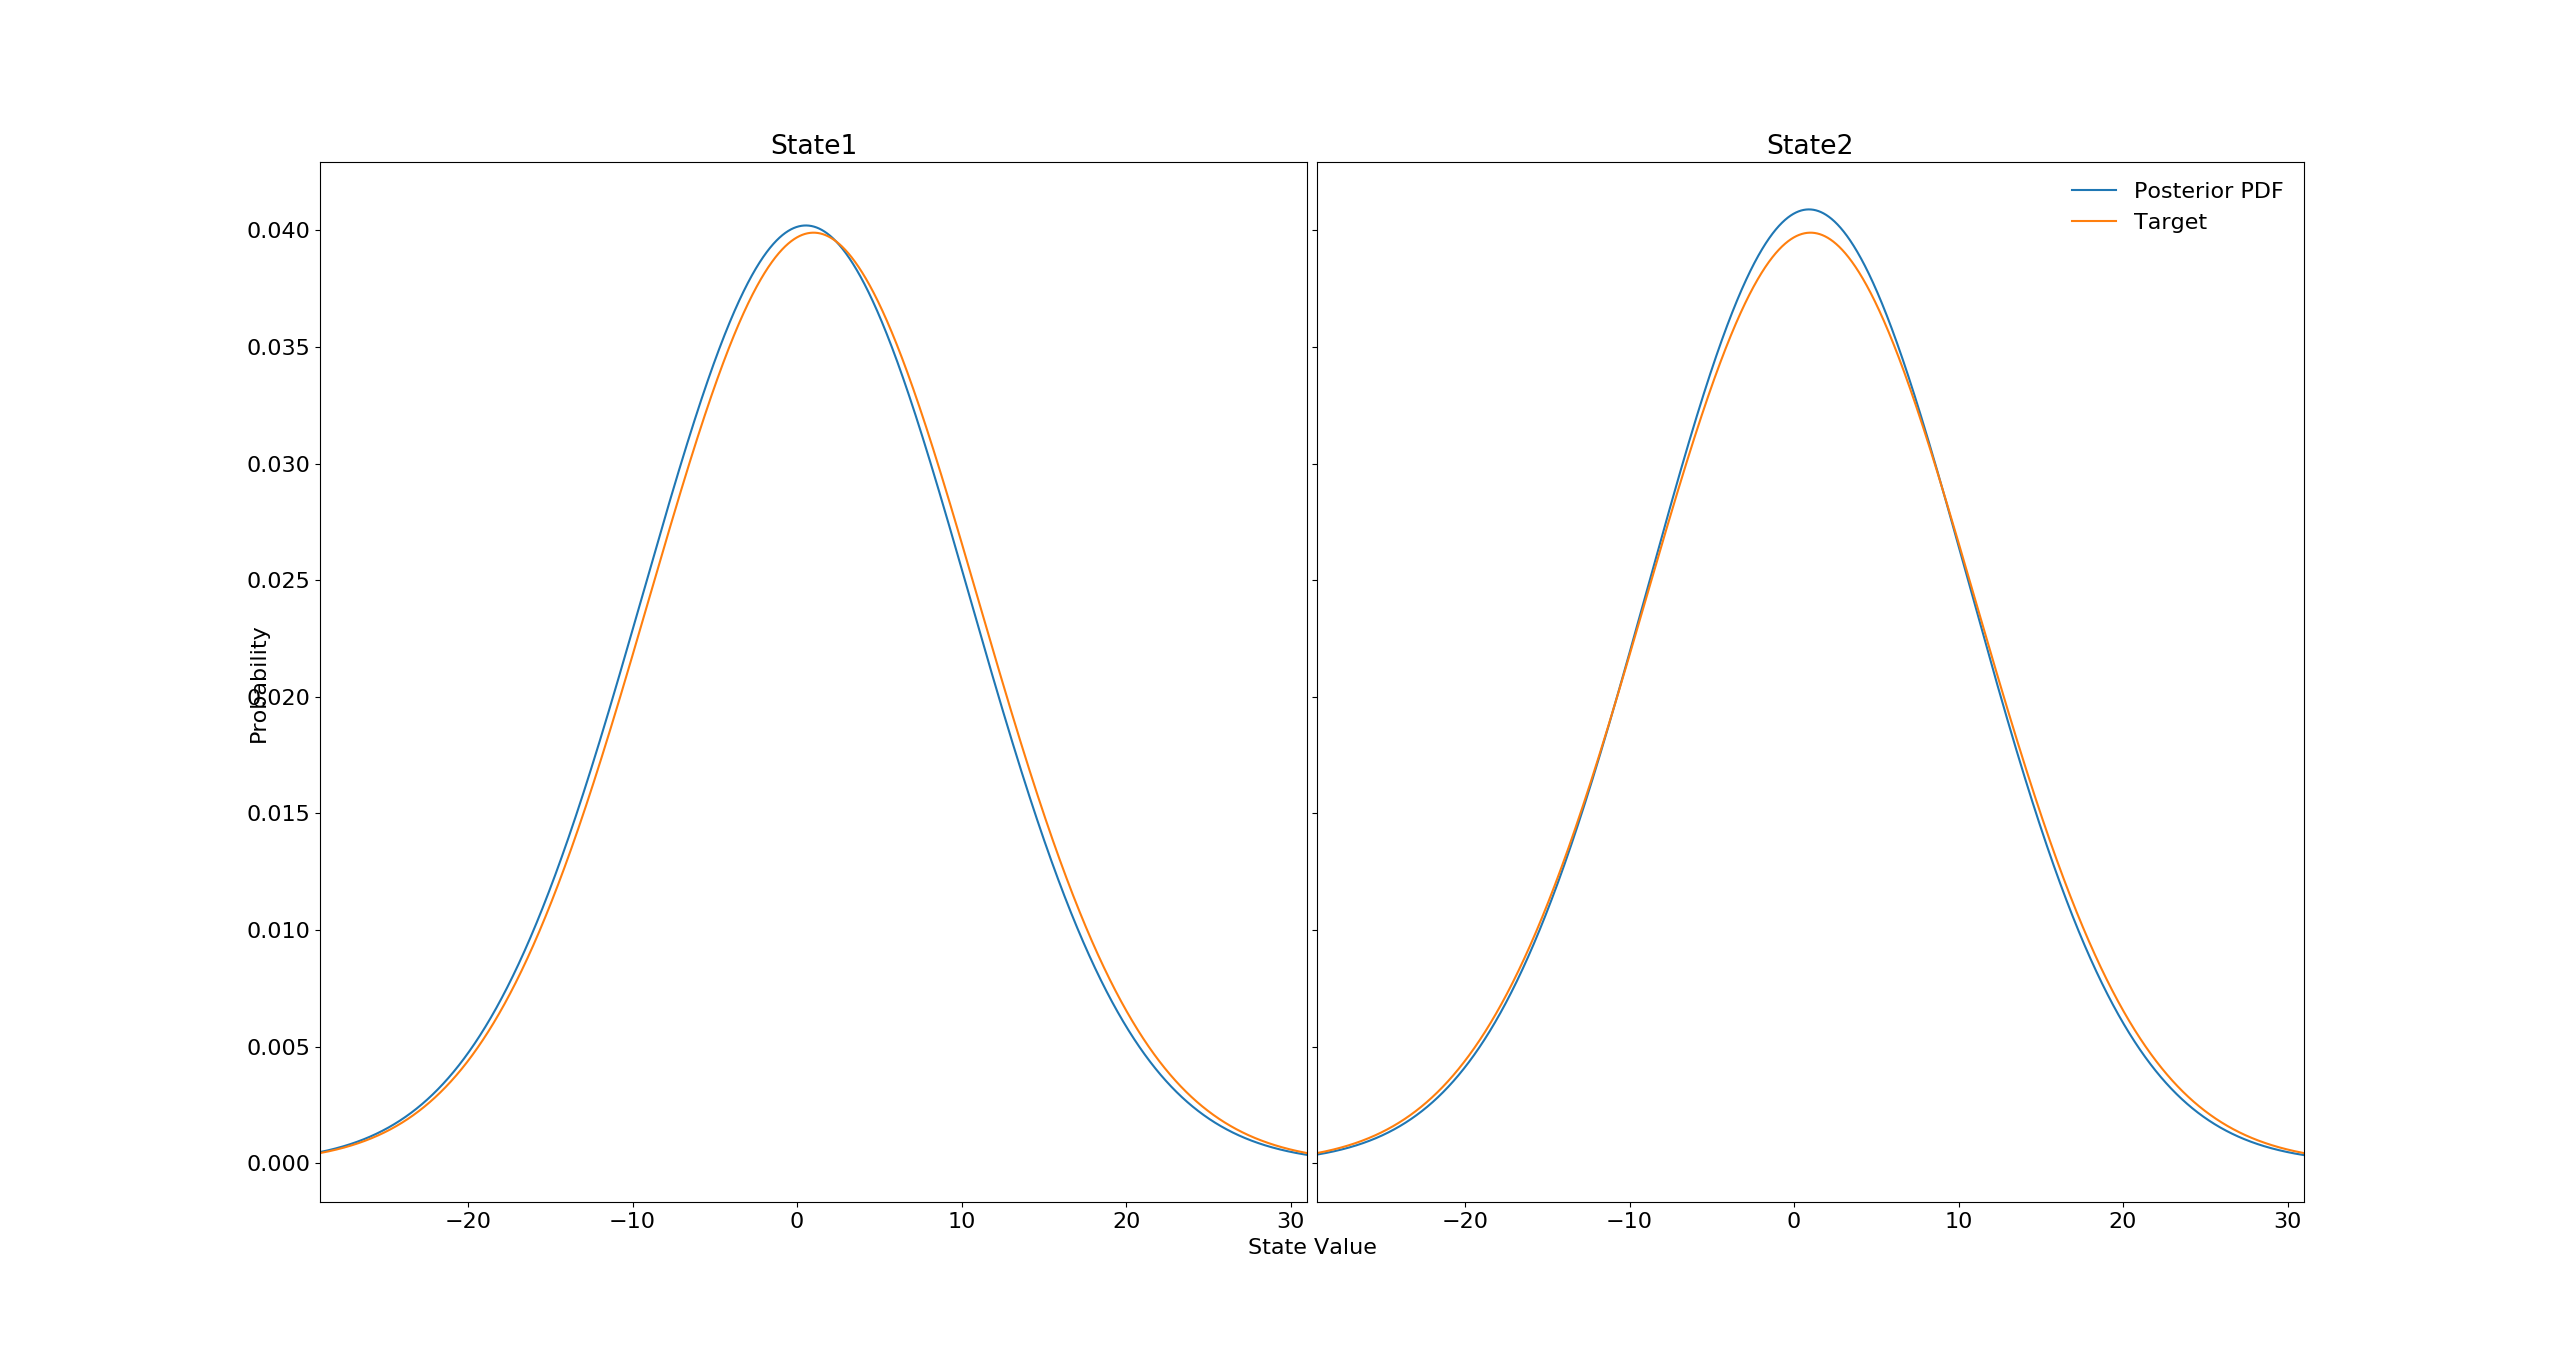
\includegraphics[width=0.5\textwidth]{3State1000iterationsSD10.png}
    }
    \\
    \subfloat[$N(1,0.1^2)$]{
        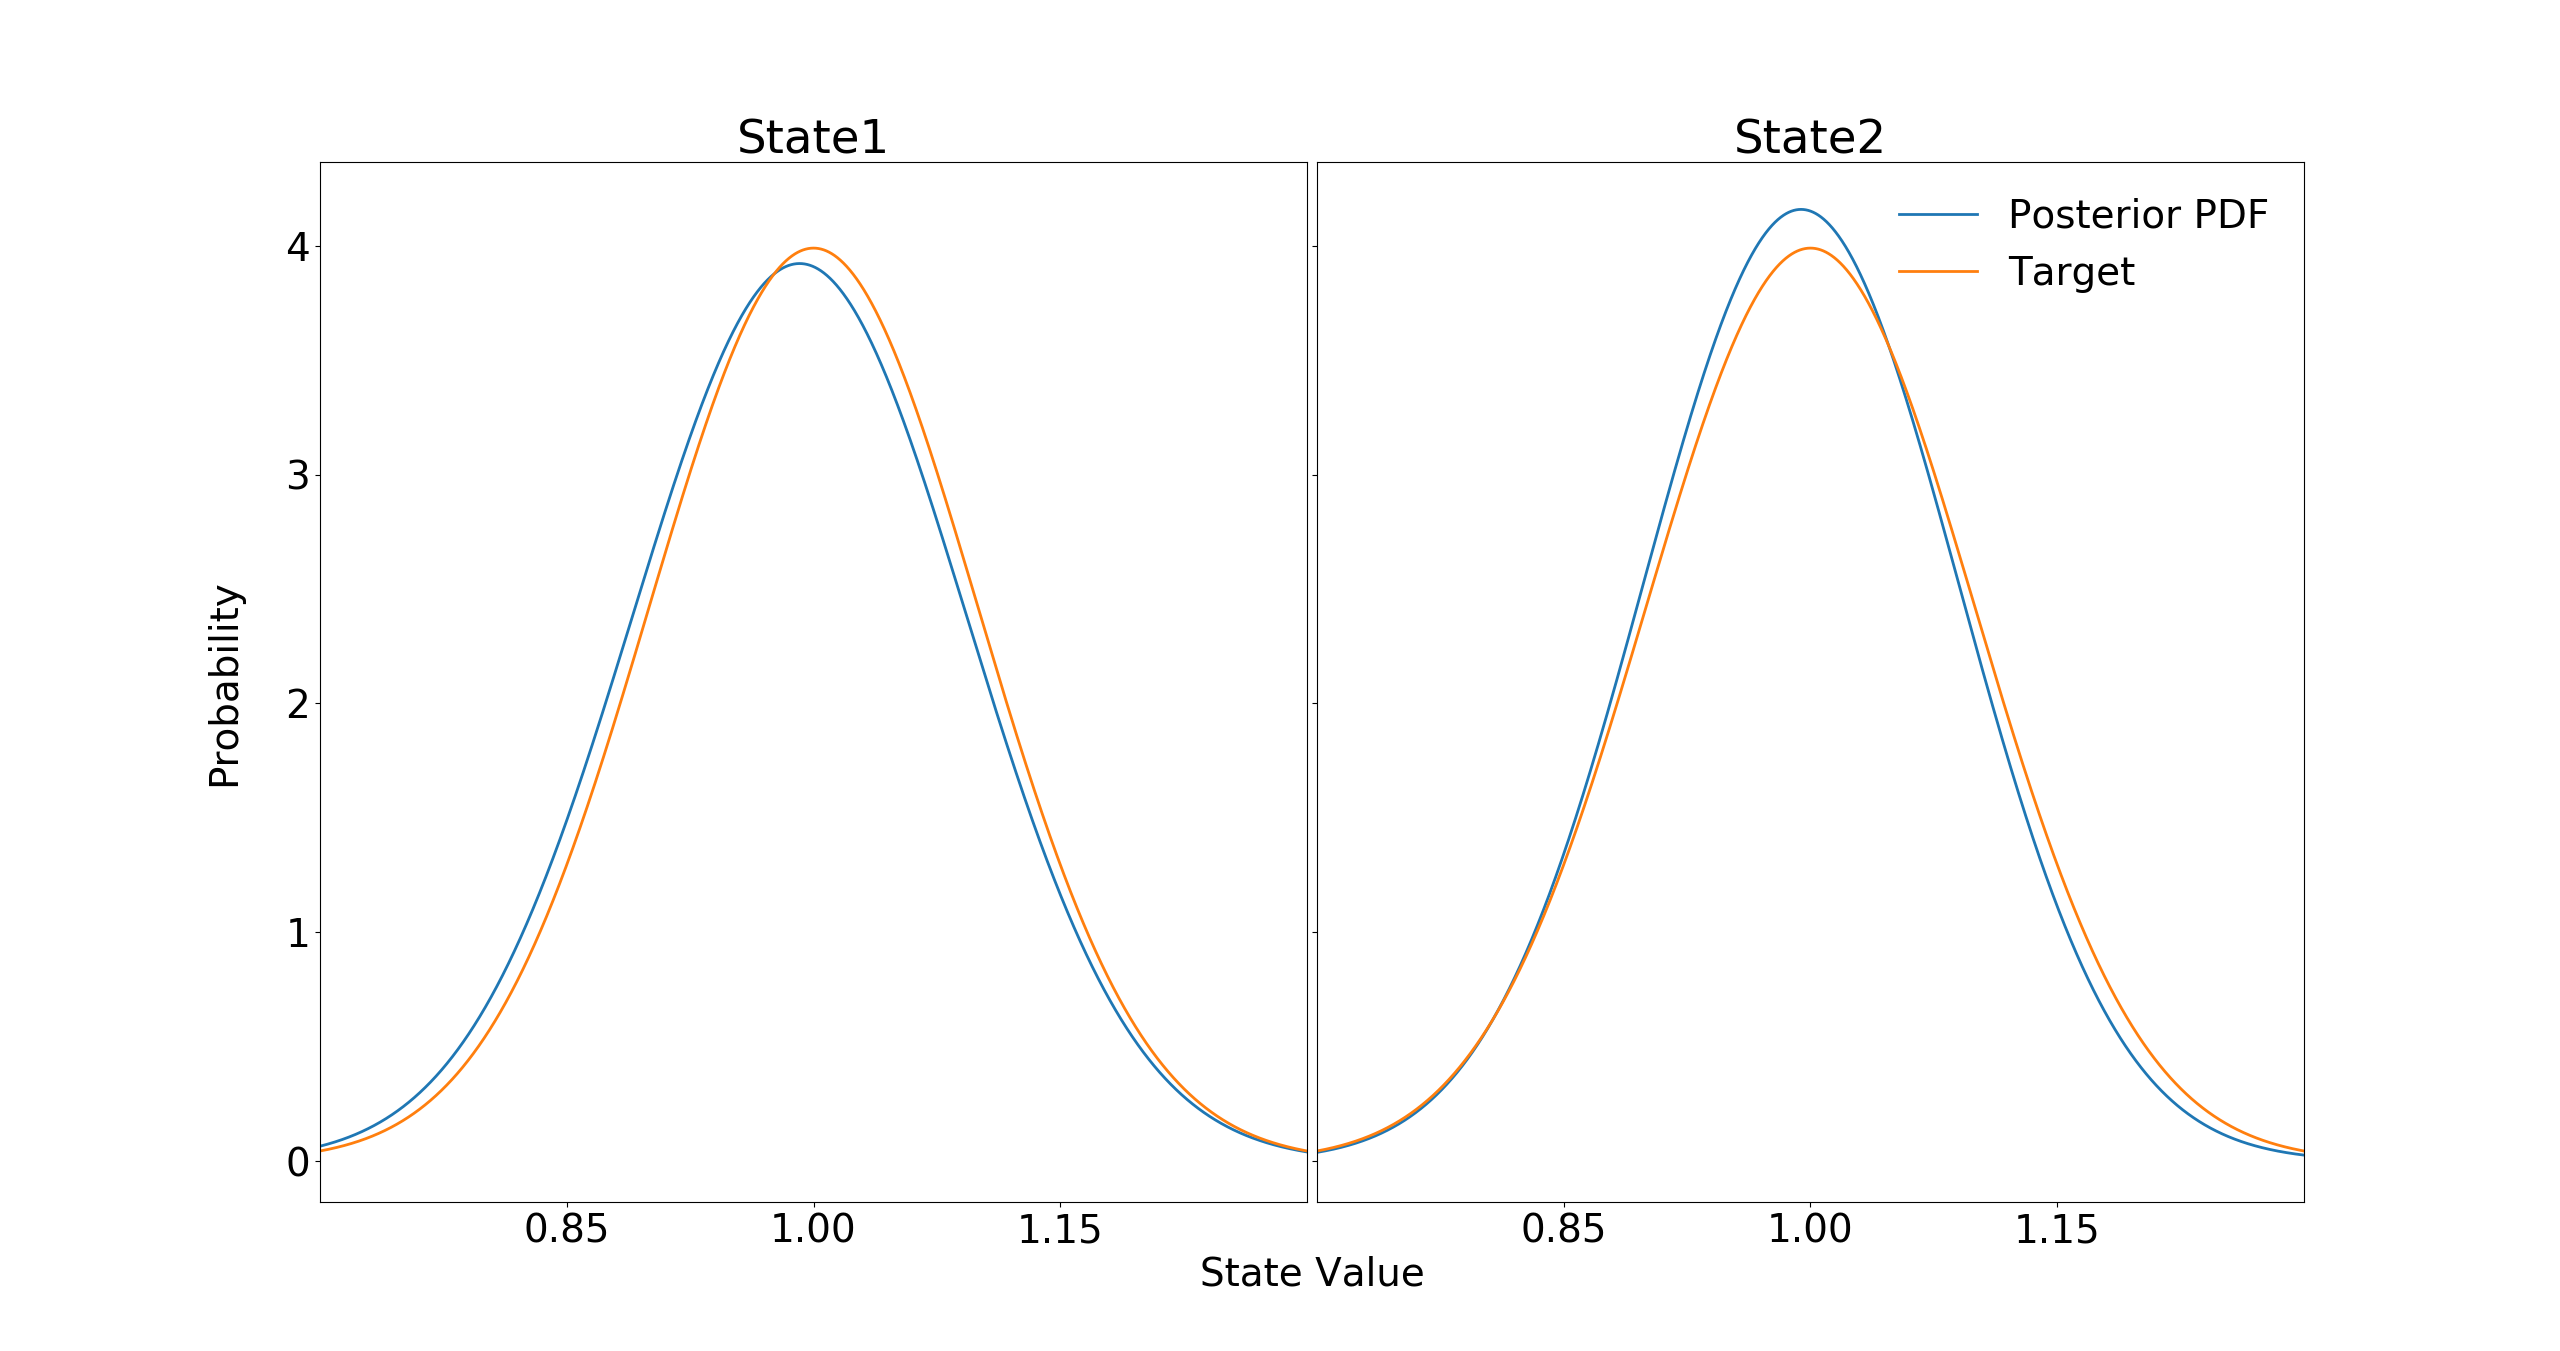
\includegraphics[width=0.5\textwidth]{3State1000iterationsSD01.png}
    }
    \subfloat[$N(1,0.01^2)$]{
        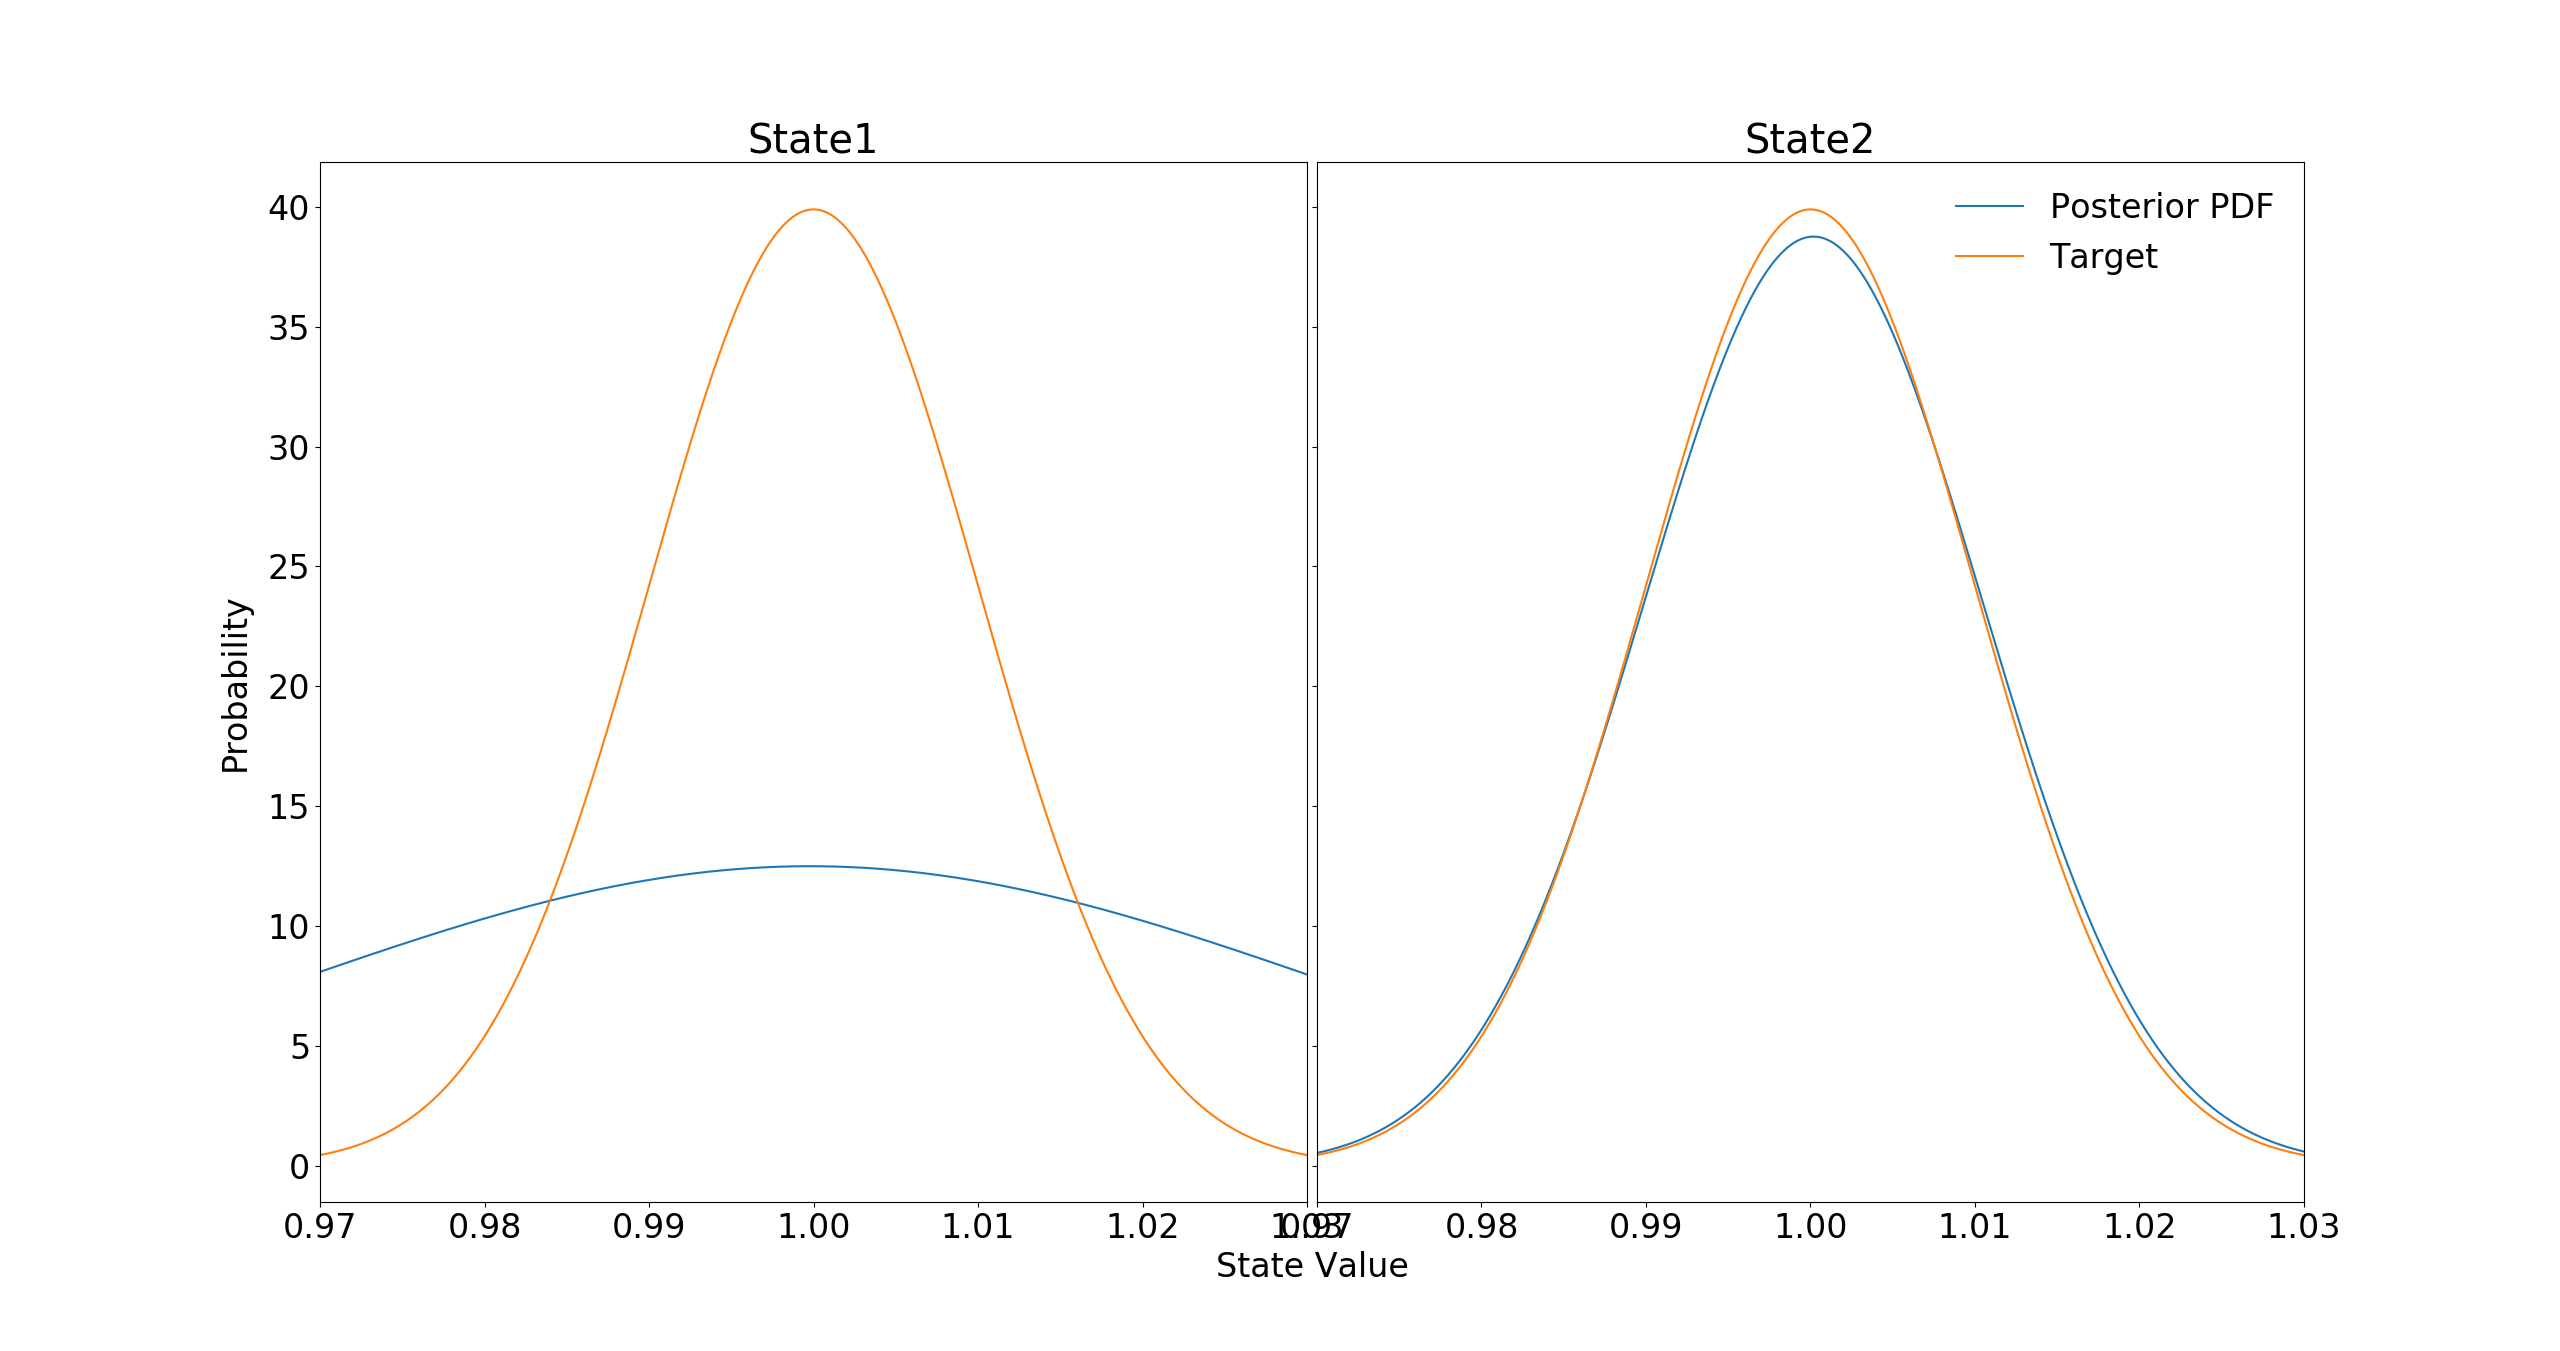
\includegraphics[width=0.5\textwidth]{3State1000iterationsSD001.png}
    }
    \caption{\textbf{Variance Propagation On 3 State Toy Example}: For larger variance targets the propagation correctly updates the state 1 variance. However the low variance targets results in an overestimation over the variance which worsens further away from the known posterior.}
    \label{fig:proptest}
\end{figure}



\subsection{\textcolor{red}{Temporary} Why sampling might not be good enough}

I've tried to get down my concerns with sampling the posterior for the target.
 
\subsubsection{Sensitivy of the Q-value}

I said at an earlier meeting that adding weak priors worked well on the chain environment. However this was a few weeks after I ran these tests, so I'd forgotten that it worked well for known noise case, but crashes for the unknown noise case. The crash is caused by samples from the weak inverse gamma prior $\text{InvGamma}(0.001, 0.001)$. This distribution can generate samples that are extremely large which causes the Q-value to explode and eventually overflow.

This can be countered by using a less weak prior but I do think it highlights the issue of using samples from the posterior when there is little data.

I think the issue is best illustrated if we consider a normal distribution. A weak normal distribution will have a large variance and spit out a wide range of values. The intuition is that this doesn't cause problems because we are as likely to sample an extremely large positive or negative number, so the magnitude cancels out.

However in a reinforcement learning setting the sample effects the next target. This means if the first sampled value is a large positive value we move the prior towards this value reducing the probability that the next target is a large negative number. To make matters worse the target is chosen to be the max value among the sampled Q-values so this effect scales with the number of actions. These factors push the Q-values to be large and leads to stability issues.

Summary: Posterior samples based on little data and weak priors lead to instability.

\section{Bayesian Deep Q Network}

\todo this section assumes DQN has been explained

The predominant issue with bayesian methods in deep reinforcement learning is using bayesian methods with neural networks. This thesis will address the linear layer method (\todo Actual name for method), a simple and computationally efficient method that comes at the cost of accuracy. 

The final layer in a DQN is a linear layer. Since bayesian regression is also a linear combination one can replace the final layer with a bayesian regression model per action. This is equivalent to rewriting the regression task to 

\begin{equation*}
	Q = \phi(X)\beta + \varepsilon \quad \text{where} \quad \varepsilon \sim N(0,\sigma^2)
\end{equation*}

where $\phi(X)$ is the neural networks output given an input $X$. Note that this means the bayesian regression no longer incorporates all the uncertainty since the above assumes no uncertainty in the $\phi(X)$ encoding. 

Training the model now needs to be split into two processes. Firstly the bayesian regression is trained using the posterior update shown above. The neural network is trained using a similar loss function as the DQN. However the networks Q-value estimate is replaced by the MAP estimate of $\beta$ resulting in

\begin{equation*}
	\theta = \theta - \alpha\nabla_\theta\big(Q_t - [\mu_n^T\phi_\theta(x_t)]\big)^2.
\end{equation*}

Note that these do not have to happen sequentially. In \cite{azziz_2018} and this implementation the bayesian regression is updated less often than the neural network.

Finally to deal with the fact that reinforcement learning is a non-stationary problem the the bayesian regression is trained for scratch each time it is updated.

\cleardoublepage